\subsubsection{Caso d'uso UC8.2.4: Modifica domanda vero/falso}
	\label{UC8.2.4}
	\begin{figure}[h]
		\centering
			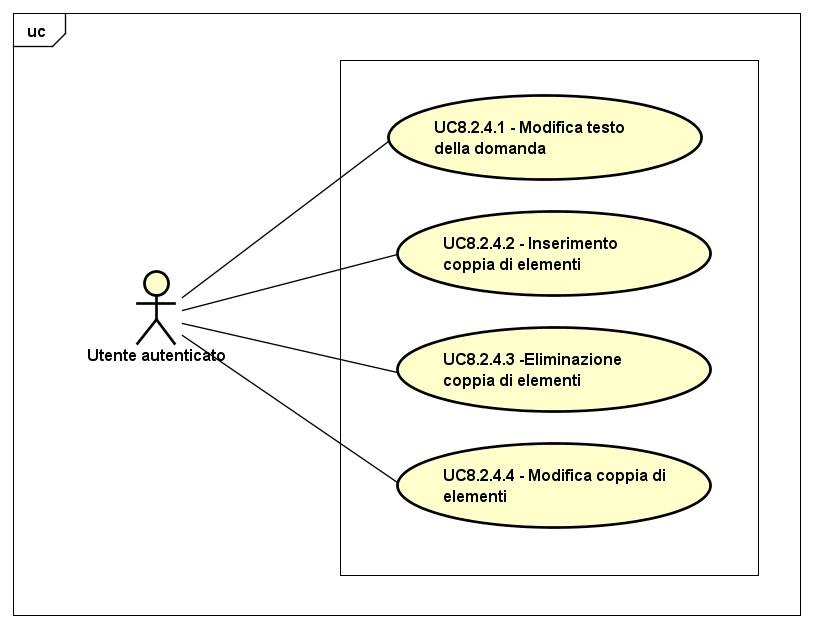
\includegraphics[scale=0.45,keepaspectratio]{UML/UC8_2_4.png}
		\caption{UC8.2.4: Modifica domanda vero/falso}
	\end{figure}
	\FloatBarrier
	\begin{itemize}
		\item
			\textbf{Attori}: utente autenticato, utente autenticato pro;
		\item		
			\textbf{Descrizione}: l'attore può utilizzare la procedura guidata per la modifica di una domanda vero/falso;
		\item
			\textbf{Precondizione}: il sistema ha ricevuto dall'attore la domanda da modificare;  
		\item
			\textbf{Postcondizione}: l'attore ha modificato una domanda vero/falso;
		\item
			\textbf{Scenario principale}:
	       		\begin{enumerate}
	       			\item
	       			L'attore può modificare il testo della domanda (UC8.2.4.1);
	       			\item
	       			L'attore può modificare l'immagine relativa al testo della domanda (UC8.2.4.2);
					\item
					L'attore può modificare la risposta corretta (UC8.2.4.3).
	 			\end{enumerate}
	\end{itemize}
	
\subsubsection{Caso d'uso UC8.2.4.1: Modifica testo della domanda}
	\begin{itemize}
		\item
			\textbf{Attori}: utente autenticato, utente autenticato pro;
		\item		
			\textbf{Descrizione}: l'attore può modificare il testo della domanda;
		\item
			\textbf{Precondizione}: il sistema mostra la funzionalità di modifica di una domanda \\vero/falso; 
		\item
			\textbf{Postcondizione}: l'attore ha modificato il testo della domanda;
		\item
			\textbf{Scenario principale}: l'attore modifica il testo della domanda. 
	\end{itemize}
	
\subsubsection{Caso d'uso UC8.2.4.2: Modifica immagine}
	\begin{itemize}
		\item
			\textbf{Attori}: utente autenticato, utente autenticato pro;
		\item		
			\textbf{Descrizione}: l'attore può modificare l'immagine relativa al testo della domanda;
		\item
			\textbf{Precondizione}: il sistema mostra la funzionalità di modifica di una domanda \\vero/falso; 
		\item
			\textbf{Postcondizione}: l'attore ha modificato l'immagine relativa al testo della domanda;
		\item
			\textbf{Scenario principale}: l'attore modifica l'immagine relativa al testo della domanda. 	
	\end{itemize}
	
\subsubsection{Caso d'uso UC8.2.4.3: Modifica risposta corretta}
	\begin{itemize}
		\item
			\textbf{Attori}: utente autenticato, utente autenticato pro;
		\item		
			\textbf{Descrizione}: l'attore può modificare la selezione della risposta corretta;
		\item
			\textbf{Precondizione}: il sistema mostra la funzionalità di modifica di una domanda \\vero/falso; 
		\item
			\textbf{Postcondizione}: l'attore ha modificato la selezione della risposta corretta;
		\item
			\textbf{Scenario principale}: l'attore modifica la selezione della risposta corretta.	 			
	\end{itemize}
	
